\documentclass[11pt]{article}
\usepackage[a4paper,margin=30mm]{geometry}
\usepackage{pdfpages,hyperref,xurl}
\emergencystretch=2em
\hypersetup{hidelinks,pdfauthor={Qian QI},pdftitle={R38 Lossless Historical Annex}}
\begin{document}
\begin{center}\Large Certified Bellman Operators for Costly Policy Revision\\[1em]
\large R38: Lossless Historical Annex\\[1em]\normalsize September 24, 2026\end{center}
This annex preserves, in their entirety, the previously materialized R34 article, technical supplement, response, computation report, and recursive historical annex. Their pages follow in that order. The earlier historical annex contains the retained predecessor manuscripts, proofs, numerical studies, and original stopped-control program. Original PDF and source files also remain unchanged in the repository.

The material is historical evidence, not a claim that all earlier assertions remain current or that earlier protocol-only execution claims have been verified retrospectively. R38's current theorems, numerical declarations, and policy-class qualifications appear in its article and technical supplement. New results come from the separately archived R38 execution.

\bigskip
\noindent Preserved files: \path{ECTA_R34.pdf}, \path{SUPP_R34.pdf},
\path{RESPONSE_R34.pdf}, \path{COMPUTATION_R34.pdf}, and
\path{HISTORY_R34.pdf}.
The publication preservation ledger records their input hashes and page counts.
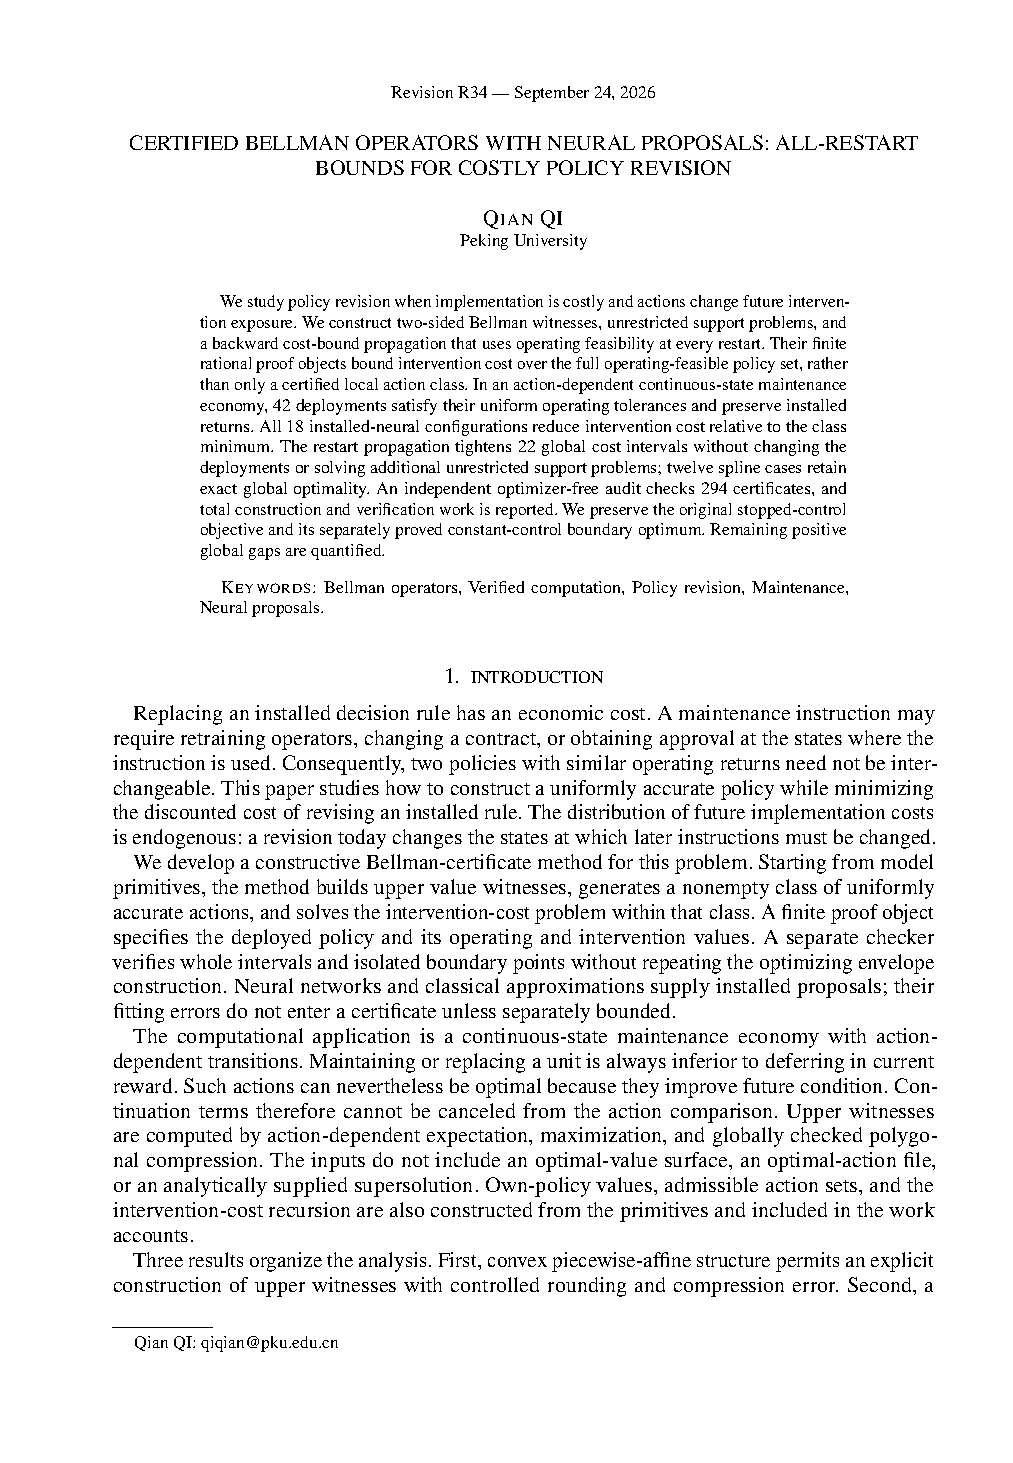
\includepdf[pages=-]{ECTA_R34.pdf}
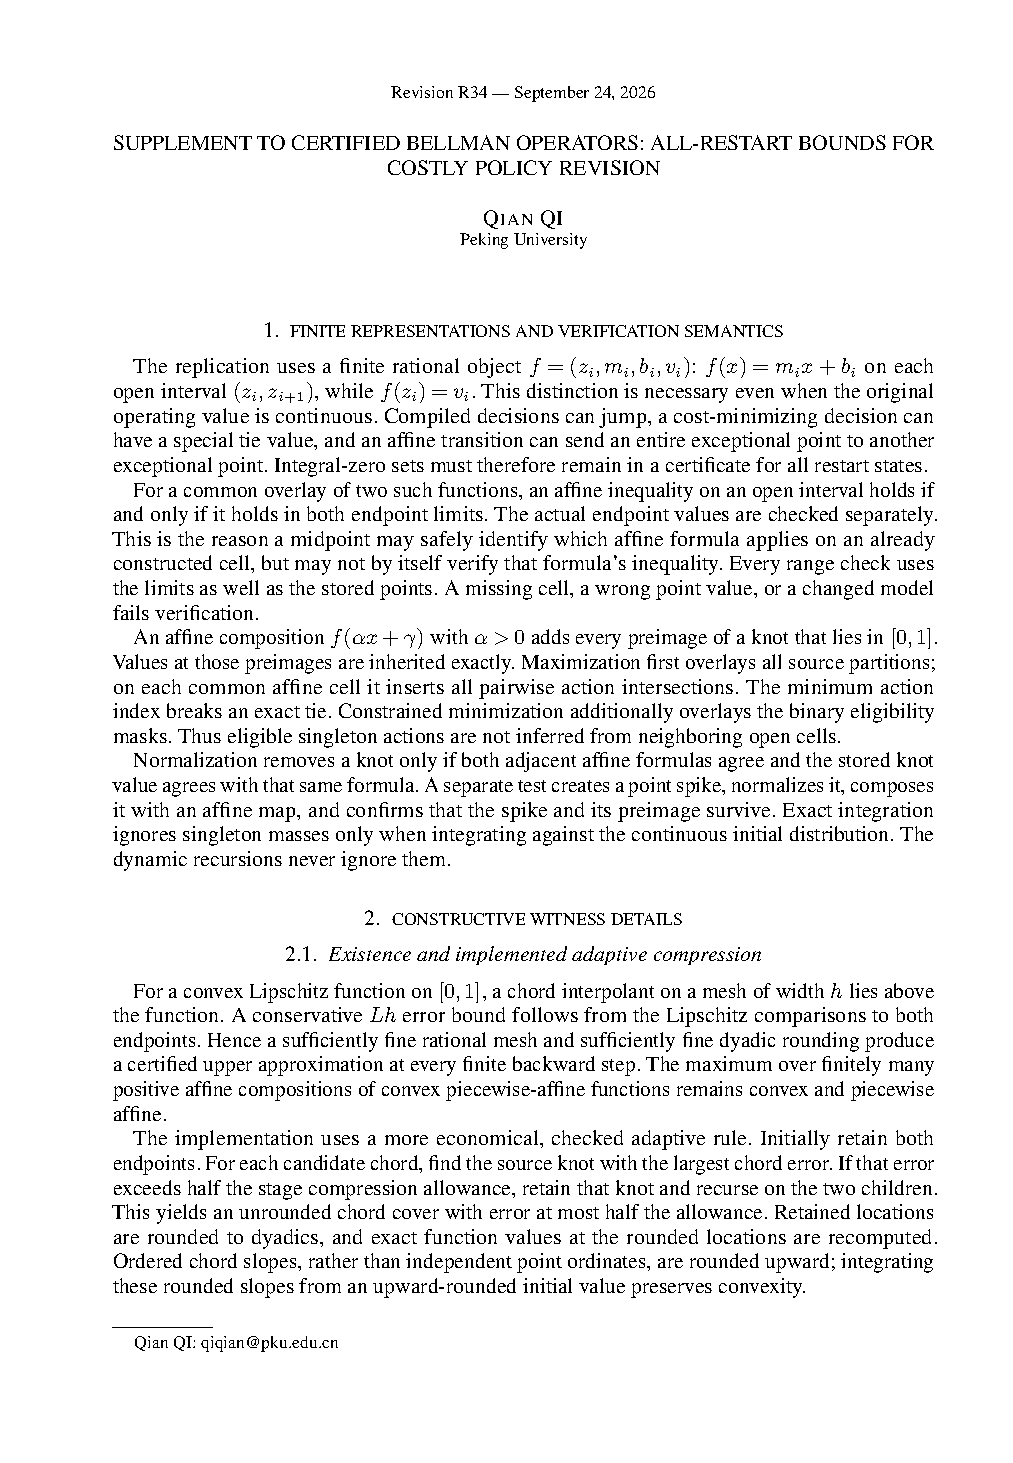
\includepdf[pages=-]{SUPP_R34.pdf}
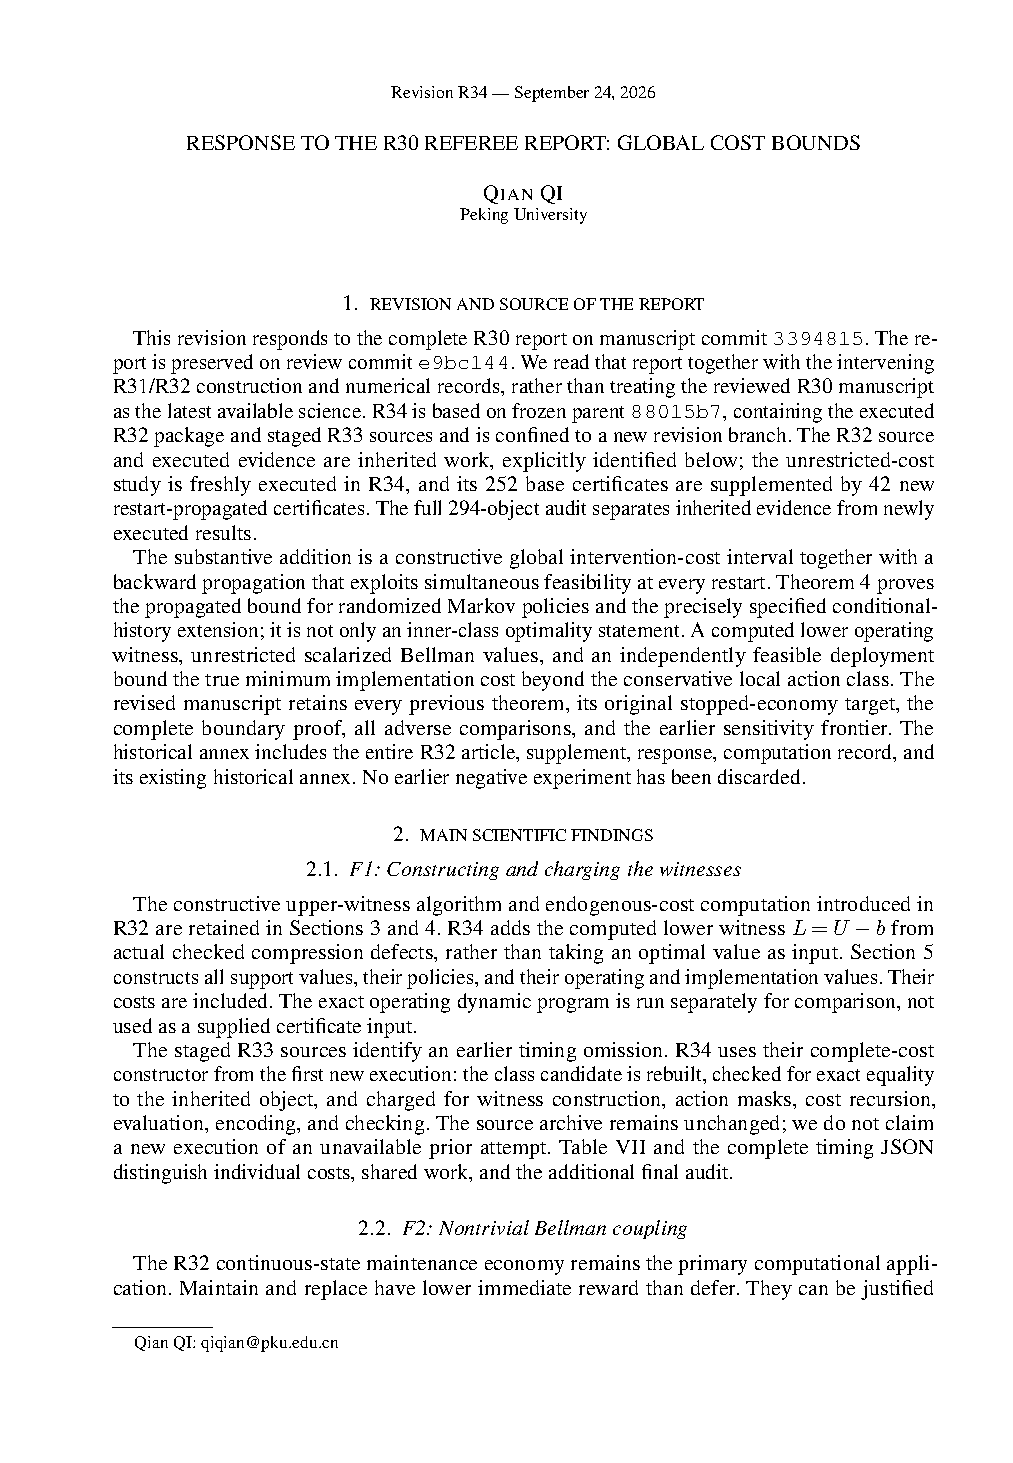
\includepdf[pages=-]{RESPONSE_R34.pdf}
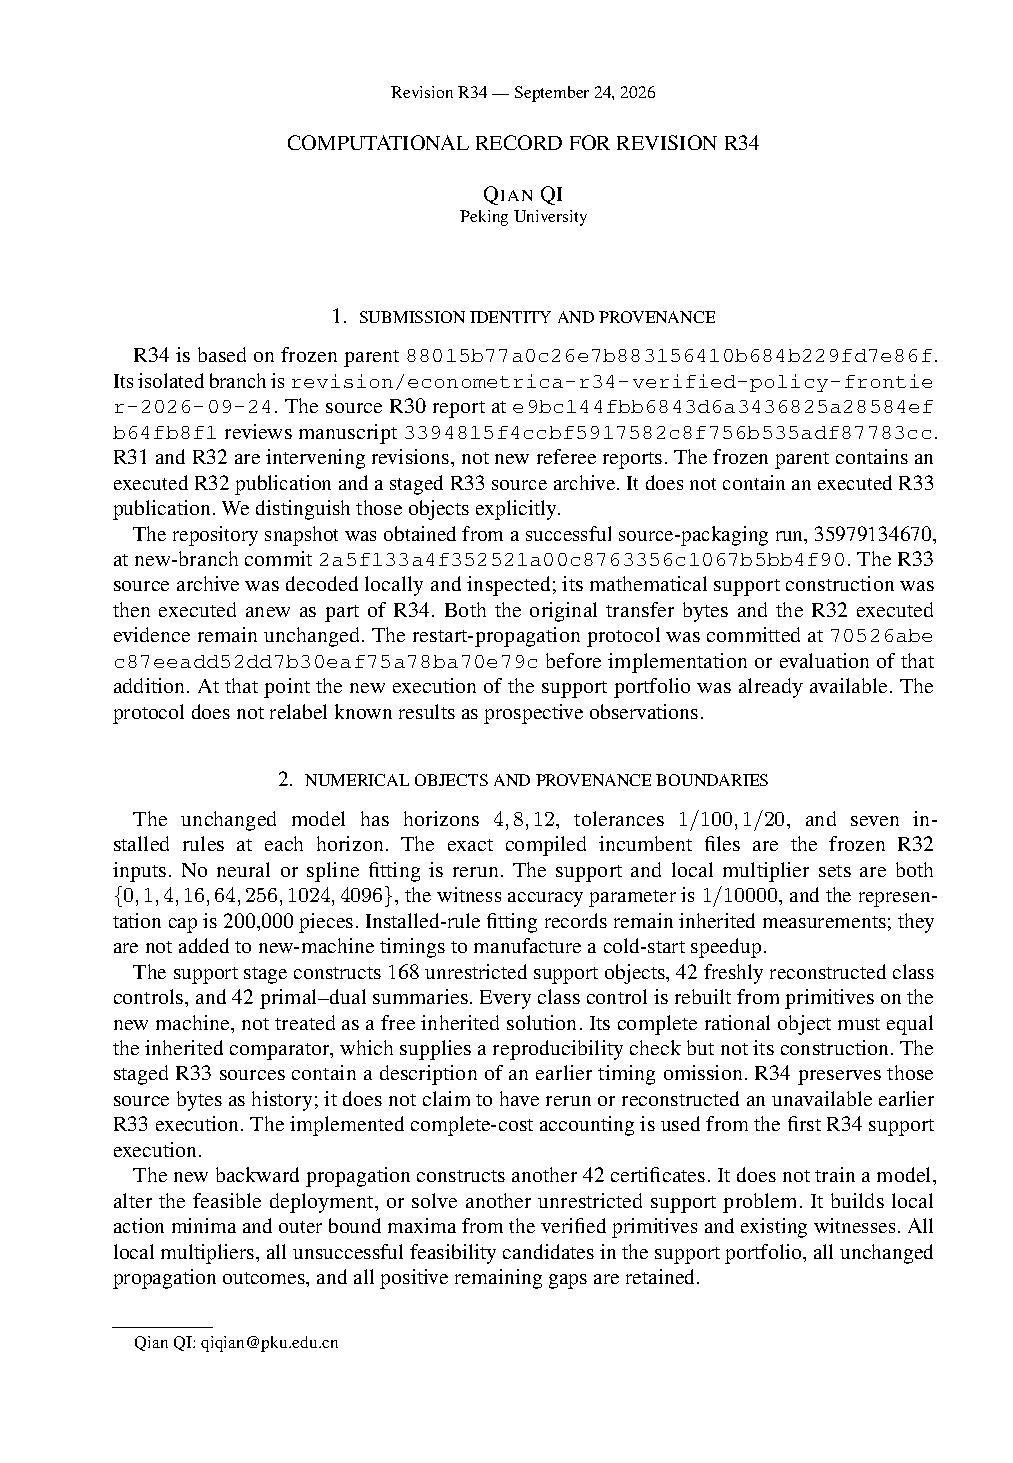
\includepdf[pages=-]{COMPUTATION_R34.pdf}
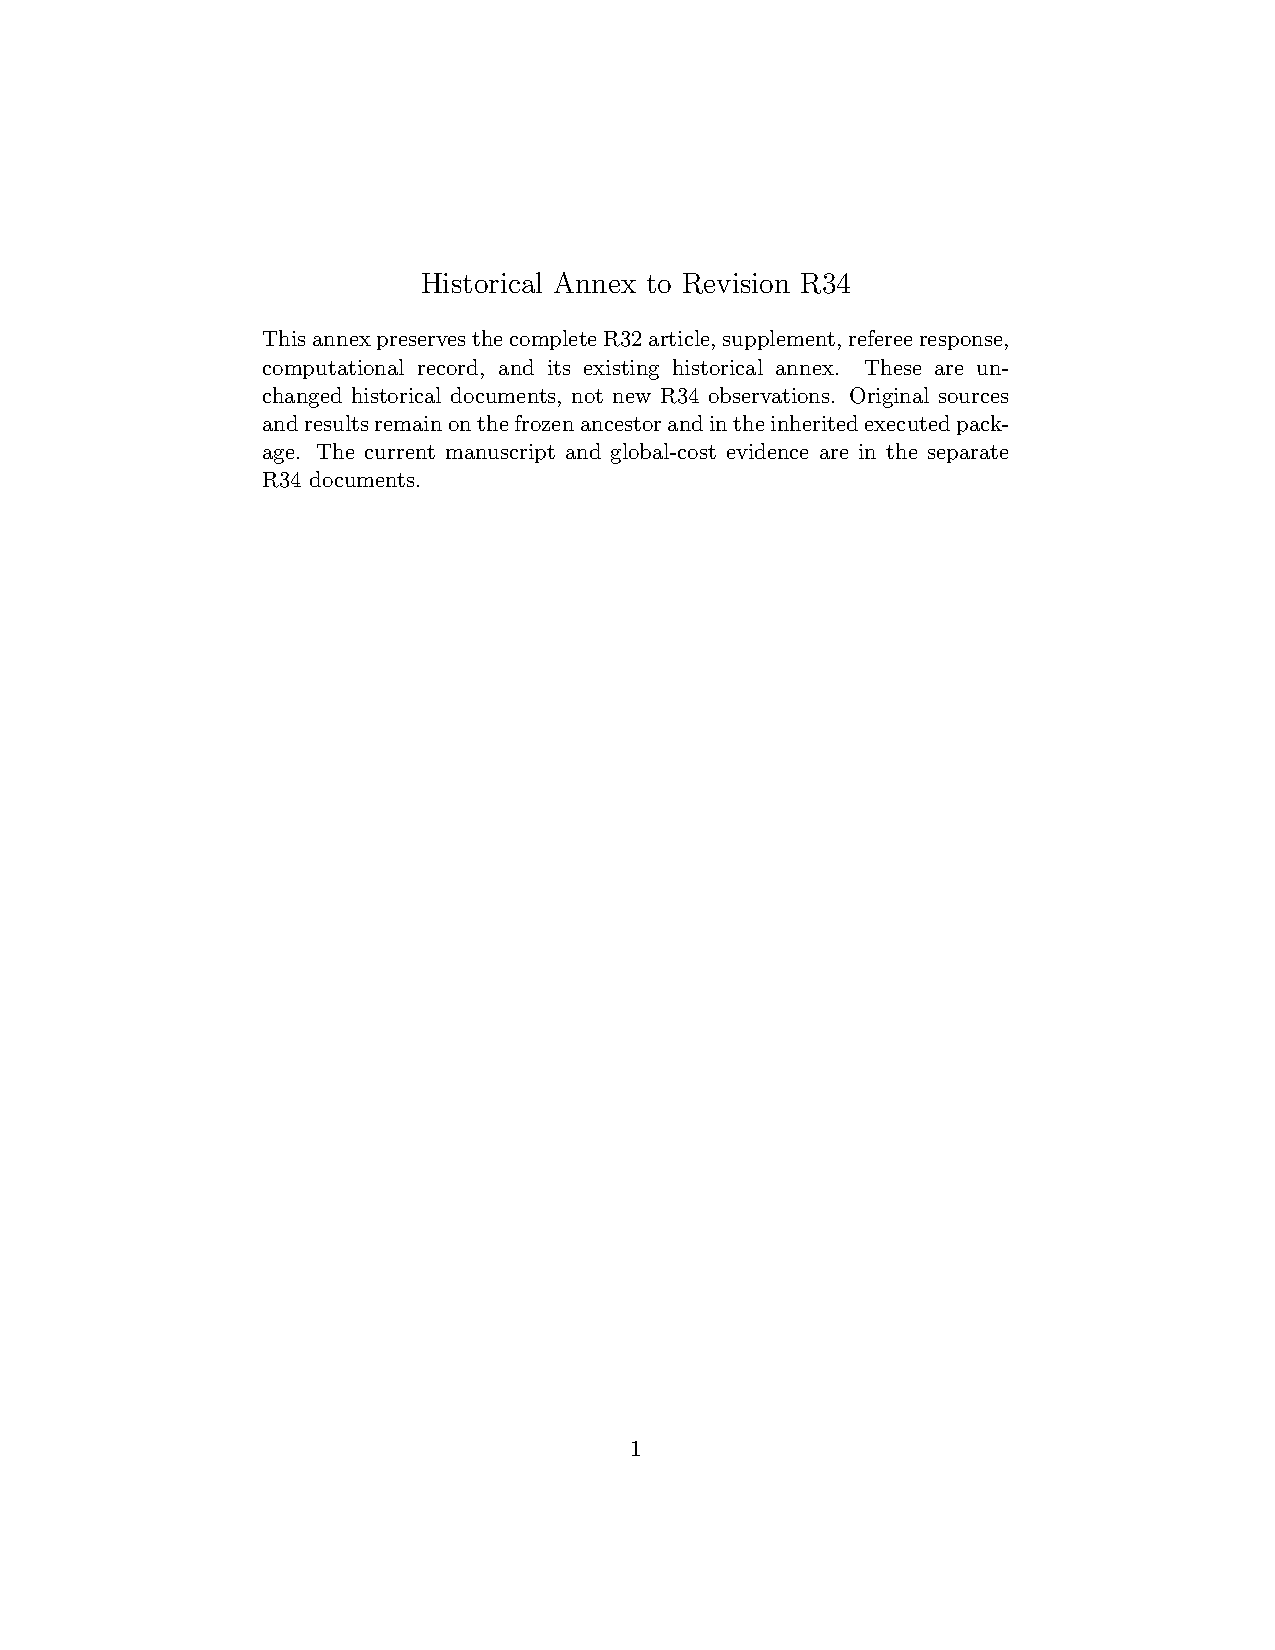
\includepdf[pages=-]{HISTORY_R34.pdf}
\end{document}
